% !TeX root = Report.tex
\documentclass[conference]{IEEEtran}
\bibliographystyle{IEEEtran}

\usepackage[none]{hyphenat}

\usepackage{color}
\usepackage{graphicx}
\usepackage{caption}
\usepackage{flafter}
\usepackage{placeins}
\usepackage{cite}
\usepackage{float}
%-------------------------------------------------------------------------------

\newcommand{\micro}{\textmu}
\newcommand{\Ohm}{$\Omega$}
\newcommand{\MATLAB}{\textsc{Matlab}\xspace}

\newcommand{\etal}       {\emph{et~al.}}
\newcommand{\ie}         {i.e.}
\newcommand{\bookcite}[2]{\cite{#1}~pg.~#2}
%-------------------------------------------------------------------------------

\newcounter{author}
\renewcommand{\theauthor}{\stepcounter{author}\raisebox{1ex}{\small\fnsymbol{author}}}
%-------------------------------------------------------------------------------

\renewcommand{\today}{%
 \number\day\space%
 \ifcase\month%
  \or January%
  \or February%
  \or March%
  \or April%
  \or May%
  \or June%
  \or July%
  \or August%
  \or September%
  \or October%
  \or November%
  \or December%
 \fi%
 \space\number\year%
}
%-------------------------------------------------------------------------------

\newlength{\TempFigureLength}
%-------------------------------------------------------------------------------

\newenvironment{FigureEnvironment}{
 \begin{figure}[!t]%
 \begin{center}%
}{
 \end{center}%
 \end{figure}%
}
%-------------------------------------------------------------------------------

\def\FigureSize{0.8}

\newcommand{\Figure}[3][scale=\FigureSize]{%
 \begin{FigureEnvironment}%
  \refstepcounter{figure}
  \addcontentsline{lof}{section}{Fig.~\thefigure{}~~~#2}
  \label{fig:#3}%
  \includegraphics[#1]{Figures/#3}\\[1em]%
  \footnotesize
  \settowidth{\TempFigureLength}{Fig.~\thefigure{}.~~{#2}}
  \ifdim \TempFigureLength > 0.95\columnwidth
   \parbox{0.95\columnwidth}{Fig.~\thefigure{}.~~{#2}}%
  \else
   Fig.~\thefigure{}.~~{#2}%
  \fi
 \end{FigureEnvironment}%
}
%-------------------------------------------------------------------------------

\newenvironment{TableEnvironment}{
 \begin{table}[H]%
 \begin{center}%
}{
 \end{center}%
 \end{table}%
}
%-------------------------------------------------------------------------------

\renewcommand{\thetable}{\Roman{table}}

\newcommand{\Table}[5]{%
 \begin{TableEnvironment}%
  \refstepcounter{table}
  \addcontentsline{lot}{section}{TABLE \thetable{}~~~#1}
  \label{tab:#5}%
  TABLE \thetable{}\\[1ex]
  \settowidth{\TempFigureLength}{\textsc{#1}}
  \ifdim \TempFigureLength > 0.95\columnwidth
   \parbox{0.95\columnwidth}{\textsc{#1}}%
  \else
   \textsc{#1}%
  \fi\\[1em]
  \renewcommand{\arraystretch}{1.2}
  \begin{tabular}{#2}
   \hline
   \hline
    #3\\
   \hline
    #4
   \hline
   \hline
  \end{tabular}
 \end{TableEnvironment}%
}
%-------------------------------------------------------------------------------

\newcommand{\Plot}[2]{
 \begin{FigureEnvironment}%
  \refstepcounter{figure}
  \addcontentsline{lof}{section}{Fig.~\thefigure{}~~~#1}
  \label{fig:#2}%
  \includegraphics[width=0.95\columnwidth]{../../Octave/Prac_1/#2}\\[1em]%
  \footnotesize
  \settowidth{\TempFigureLength}{Fig.~\thefigure{}.~~{#1}}
  \ifdim \TempFigureLength > 0.95\columnwidth
   \parbox{0.95\columnwidth}{Fig.~\thefigure{}.~~{#1}}%
  \else
   Fig.~\thefigure{}.~~{#1}%
  \fi
 \end{FigureEnvironment}%
}
\usepackage{textcomp} %Used in listings for printing upright quotes
\usepackage{listings} %For typesetting source code
\lstloadlanguages{C++, Matlab, Verilog}
%-------------------------------------------------------------------------------

\lstset{%
 frame      = single,%
 basicstyle = \tiny\ttfamily,%
 basewidth  = 1.3ex%
% basicstyle = \scriptsize\ttfamily,%
% basewidth  = 1.2ex%
}
%-------------------------------------------------------------------------------

\definecolor{keyword}{rgb}{0.5, 0.0, 0.0}
\definecolor{comment}{rgb}{0.0, 0.5, 0.0}
\definecolor{string} {rgb}{0.0, 0.0, 0.7}
\definecolor{define} {rgb}{1.0, 0.5, 0.0}
\definecolor{string2}{rgb}{0.5, 0.0, 0.5}
%-------------------------------------------------------------------------------

\newcounter{Listing}
\renewcommand{\theListing}{\arabic{Listing}}

\newlength{\CodeWidth}

\newcommand{\StartListing}[2]{
 \setlength{\CodeWidth}{0.95\columnwidth}
 \figure[!t]
 \refstepcounter{Listing}
 \addcontentsline{lof}{section}{Listing \theListing{}~~~#1}
 \label{lst:#2}
 \def\ListingCaption{#1}
 \noindent\centering\minipage{\CodeWidth}%
}
\newcommand{\EndListing}{
 \endminipage\\%
 {%
  \footnotesize%
  \settowidth{\TempFigureLength}{Listing~\theListing{}.~~\ListingCaption}%
  \ifdim \TempFigureLength > 0.95\columnwidth%
   \parbox{0.95\columnwidth}{Listing~\theListing{}.~~\ListingCaption}%
  \else%
   Listing~\theListing{}.~~\ListingCaption%
  \fi%
 }%
 \endfigure%
}

\newcommand{\StartListingInline}{%
 \setlength{\CodeWidth}{0.95\columnwidth}%
 \noindent\centering\minipage{\CodeWidth}%
}
\newcommand{\EndListingInline}  {\endminipage\par}
%-------------------------------------------------------------------------------

\newcommand{\SetupMatlab}{
 \lstset{%
  language         = Matlab,%
  upquote          = true,%
  showstringspaces = false,%
  keywordstyle     = {\color{keyword}\slshape},%
  commentstyle     = {\color{comment}},%
  stringstyle      = {\color{string}},
  morecomment      = [l][\color{comment}]{\#}%
 }%
}

\lstnewenvironment{Matlab_float}[2]{
 \SetupMatlab
 \StartListing{#1}{#2}
}{
 \EndListing
}

\lstnewenvironment{Matlab}{
 \SetupMatlab
 \StartListingInline
}{
 \EndListingInline
}
%-------------------------------------------------------------------------------

\newcommand{\SetupGLSL}{
 \lstset{%
  language=C,%
  upquote=true,%
  showstringspaces=false,%
  keywordstyle=   {\color{keyword}\slshape},%
  commentstyle=   {\color{comment}},%
  stringstyle =   {\color{string}},%
  morecomment =[l][\color{define}]{\#},%
  morekeywords={%
   in,%
   out,%
   vec2,%
   vec3,%
   vec4,%
   sin,%
   length,%
   texture2D,%
   sampler2D,%
   gl_FragColor,%
   varying,%
   uniform,%
   discard%
  }%
 }%
}

\lstnewenvironment{GLSL_float}[2]{
 \SetupGLSL
 \StartListing{#1}{#2}
}{
 \EndListing
}

\lstnewenvironment{GLSL}{
 \SetupGLSL
 \StartListingInline
}{
 \EndListingInline
}
%-------------------------------------------------------------------------------

\newcommand{\SetupOpenCL}{
 \lstset{%
  language=C,%
  upquote=true,%
  showstringspaces=false,%
  keywordstyle=   {\color{keyword}\slshape},%
  commentstyle=   {\color{comment}},%
  stringstyle =   {\color{string}},%
  morecomment =[l][\color{define}]{\#},%
  morekeywords={%
   __kernel,%
   __global,%
   __local,%
  get_global_id%
  }%
 }%
}

\lstnewenvironment{OpenCL_float}[2]{
 \SetupOpenCL
 \StartListing{#1}{#2}
}{
 \EndListing
}

\lstnewenvironment{OpenCL}{
 \SetupOpenCL
 \StartListingInline
}{
 \EndListingInline
}
%-------------------------------------------------------------------------------

\newcommand{\SetupVerilog}{
 \lstset{%
  language=Verilog,%
  upquote=true,%
  showstringspaces=false,%
  keywordstyle=   {\color{keyword}\slshape},%
  commentstyle=   {\color{comment}},%
  stringstyle =   {\color{string}},%
  morecomment =[l][\color{define}]{`}%
 }%
}

\lstnewenvironment{Verilog_float}[2]{
 \SetupVerilog
 \StartListing{#1}{#2}
}{
 \EndListing
}

\lstnewenvironment{Verilog}{
 \SetupVerilog
 \StartListingInline
}{
 \EndListingInline
}
%-------------------------------------------------------------------------------

\newcommand{\SetupCpp}{
 \lstset{%
  language         = C++,%
  upquote          = true,%
  showstringspaces = false,%
  keywordstyle     = {\color{keyword}\slshape},%
  commentstyle     = {\color{comment}},%
  stringstyle      = {\color{string}}%
 }%
}

\lstnewenvironment{Cpp_float}[2]{
 \SetupCpp
 \StartListing{#1}{#2}
}{
 \EndListing
}

\lstnewenvironment{Cpp}{
 \SetupCpp
 \StartListingInline
}{
 \EndListingInline
}
%-------------------------------------------------------------------------------

\usepackage[pdftex                       ,%
            bookmarks         = true     ,%
            bookmarksnumbered = true     ,%
            setpagesize       = false    ,%
            colorlinks        = true     ,%
            linkcolor         = black    ,%
            urlcolor          = black    ,%
            citecolor         = black    ,%
            pdfpagelayout     = OneColumn,%
            pdfstartview      = FitH]{hyperref}
%-------------------------------------------------------------------------------

%-------------------------------------------------------------------------------


\title{Prac5: Trigger Surround Cache}

\author{%
 \setcounter{author}{1}
 \IEEEauthorblockN{Cameron F Clark\theauthor\ and Kian S Frassek\theauthor}
 \setcounter{author}{1}
 \IEEEauthorblockA{%
  EEE4120F Class of 2024\\
  University of Cape Town\\
  South Africa\\
  \theauthor{}CLRCAM007~~\theauthor{}KIAFRS001\\
 }
}

\begin{document}
\begin{sloppypar}

    \maketitle

    % We're using separate files for each main section
    % Please see the subdirectories Body/.. for the files.

    %\begin{abstract}
\end{abstract}


    \section{Introduction}
A Field Programmable Gate Array (FPGA) is an interconnected circuit which can be coding using Verilog and can be customized for specific applications.
This project details the building of a simple Trigger Surround Cache (TSC) using an ADC and a ring buffer memory device; an ADC records an input analog signal and converts it to a digital signal.
A ring buffer is a type of storage method where you have a fixed size storage, and you have two pointers: a read pointer which is also called the head and a write pointer which is also called the tail.
The TSC will also be able to communication with other devices using a clocked serial data transfer protocol.

    \section{Design and Implementation }

\subsection{Hardware ans Software}
This was run on a MacBook Pro computer using Iverilog. Additionally, gtkwave was used to monitor the wires.

\subsection{TSC design overview}

The TSC (Trigger Surround Cache) has a 3 bit state register, a 32-bit timer,
a 32-bit TRIGGER\_TM, and an internal ring buffer.
It is connected to the ADC (Analog-to-Digital Converter)
via a request (REQ), ready (RDY), and data (DAT) lines.
Additionally, the TSC can communicate with other devices using triggered (TRD), Send Buffer (SBF),
serial data (SD), and completed data (CD) registers and wires.


\begin{figure}[H]
      \centering
      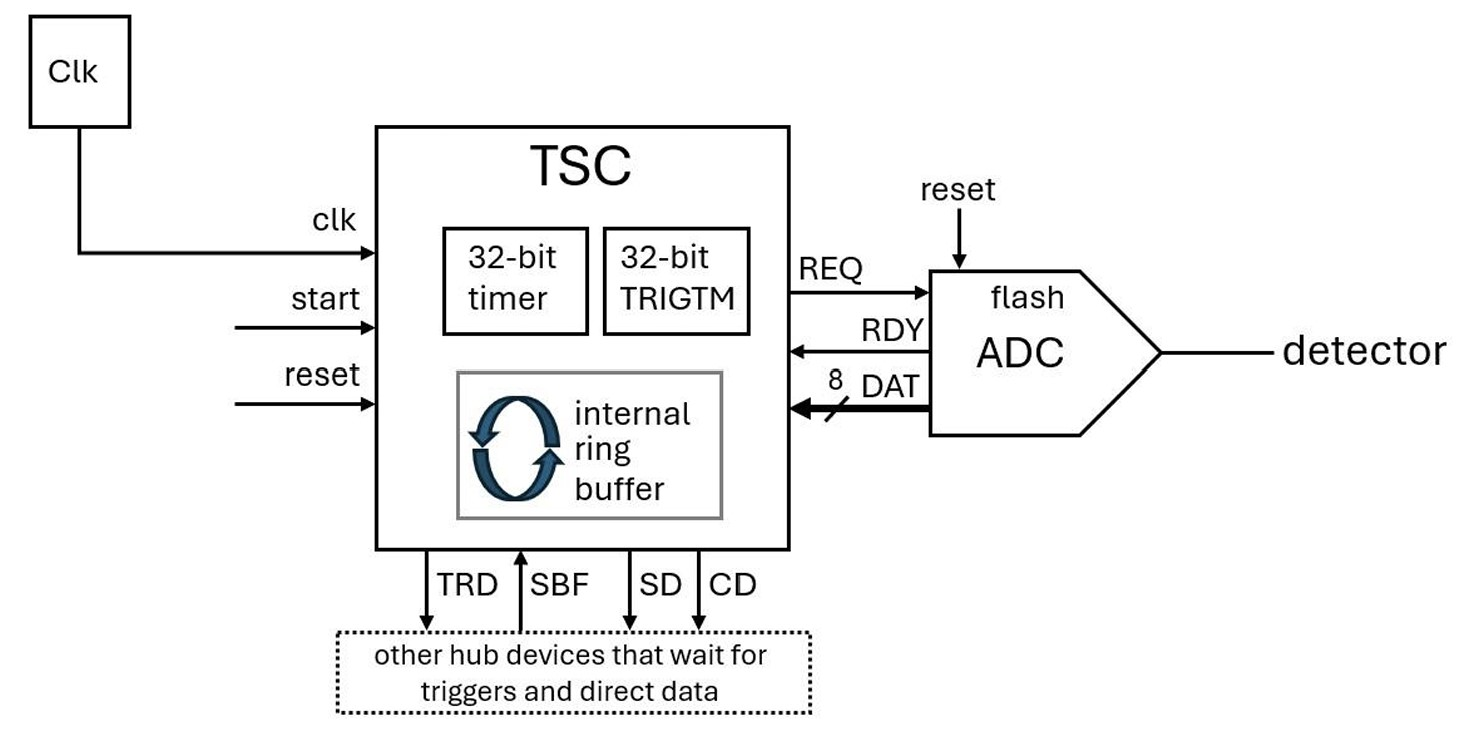
\includegraphics[width=0.8\columnwidth]{Figures/block_diagram_of_TSC}
      \caption{Block diagram of the TSC}
      \label{fig:block diagram of TSC}
\end{figure}

There is also an accompanying TSC\_tb test bench which is used to initiate and test the TSC module.

\subsection{CLock (clk)}
A 250 MHz clock signal is set up on clk wire in the TS\_tb test bench.

\subsubsection{State register}
The state register is a 3-bit register that has the folowing states:
\begin{itemize}
      \item 000 Stop :
            State when the machine is powered on and has not been reset yet.
      \item 001 ready :
            State that is enter on the reset pin rising edge and it waits for the start pin rising edge.
      \item 010 Running :
            State that is entered from ready or Idle state once the start pin rising edge is pulled hight.
            It incrementing the timer and wright adc values to the ring buffer.
      \item 011 Triggered :
            State entered when the value read from the ADC is
            greater than the predetermined trigger value (TRIGVL).
            It capturing the next 16 values.
      \item 100 IDLE ;
            This state is entered when a trigger event has occurred
            and the TSC is waiting for the start pin or SPF pins rising edge.
      \item 101 SENDING :
            This state is entered from the IDLE state when the SFB gose high. It indicates that data is being sent on the SD line.
\end{itemize}


\subsubsection{Timer}
The timer is incremented on the rising edge of the clock. When
a trigger even occurs the timer is save in the TRIGTM register which is outputted to the test bench.
The timer is reset if a transition into a running state occurs.
To calculate the time store in the TRIGTM register the timer is multiplied by the clock period (4 ps).



\subsubsection{Ring Buffer}
The ring buffer is used to store the values read by the ADC.
It is made up of 32 8-bit registers stored in an array called ring\_buffer.
The tail pointer is named write\_prt and is Initial set to 5'b11111.
and the head pointer is named read\_ptr and is initial set to 5'b00000.
The 5 bit format for the head and tail index is used to induce role offer at value 32 (32 just becomes 0).
To add a new value to the ring buffer the write\_ptr is incremented and then the
value is stored in the ring buffer at the write\_ptr index then read\_ptr is incremented.
To read a value from the ring buffer the value at the read\_ptr index is read and the read\_ptr is incremented.
this proses is repeated until the read\_prt = wright\_ptr. Indicates that all the values have been read.

\subsubsection{How the TSC intervacec with the ADC}
The ADC is initialized in the TSC module. this is creates the adc\_request, adc\_request,  adc\_ready, and DAT wires.
The adc\_request line is to the main reset line this mean that the ADC is reset when the TSC\_td module pulls the reset pin hight.
once the ADC is reset the adc\_ready line is pulled hight to indicate that the ADC is ready to send data.
When the TSC module detects the adc\_ready line is hight and the TSC is in the running state.
The TSC will pull the adc\_request line hight on  the posedge of the clk line for 1 ps to request data from the ADC. This can be seen in the two code section below.

\begin{lstlisting}[language=Verilog, caption={Code for storing data and moving pointers i the posedge adc\_ready}]
      always @(posedge adc_ready) begin
            if (adc_request) begin
            #1 //delay so the pulse doesn't disappear on the echo. TO BE REMOVED
          
            //manage trigger_value
            //... the trigger code is here

      //store data and move pointers around
      ring_buffer[++write_ptr] = adc_data;
      read_ptr++;

      adc_request = 0; //pull request down
    end
  end
\end{lstlisting}

\begin{lstlisting}[language=Verilog, caption={Code for requesting data from the ADC on posedge of the clock when in RUNNING state}]
      `RUNNING: begin
        timer++;
        if (~ adc_request)
          adc_request = 1; //request new adc value (handled with posedge adc_ready)
      end
\end{lstlisting}















    \section{Testing and Validation}
This section details the tests that were conducting on the TSC module while it is connected to the ADC and HUB module.
The tests conducted were only aimed to prove the functionality of the module and weren't aimed to test the module protection of misuse, even-though the TSC module was written to handle such cases.

The test bench runs a simple test of sending a pulse on the reset line followed by a pulse on the start line to move the module into running mode.
The module will next get triggered by one of the 256 ADC values going above the TRIGVL.
The TRIGVL is set at 0xC8 and there are only two values in the ADC csv file which are above 0xC0 which are the 150th and 200th values.
The test bench is programmed to send a start pulse on the first trigger and an SBF pulse on any subsequent triggers.

The test was run as one continuous test and several snippets of gktwave were taken and explained in chronological order.

\subsection{Reseting and Starting}
\begin{figure}[H]
    \centering
    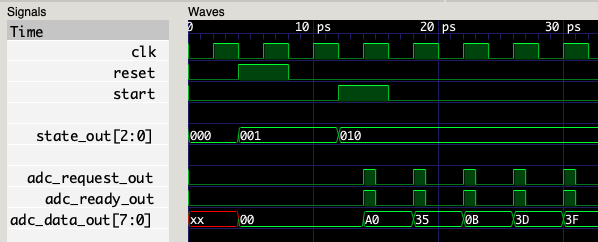
\includegraphics[width=\columnwidth]{Figures/Areset_start_adc}
    \caption{Resetting and Starting gktwave Output}
    \label{fig:testA}
\end{figure}

Firstly, a reset then start pulse are sent and the TSC module response by changing the state from STOP (0b000) to READY (0b001) and then to RUNNING (0b010).
Once the module has entered running mode, it correctly requests data from the the ADC module every rising clock edge, and the adc replies by pulling the ready line high and outputs a new byte on the data bus.
In a real world implementation of this there would be a slight delay between the request being pulled high and the ready begin pulled high.
Next, the TSC module acknowledges the adc ready and resets the request line.
Again, in a real world implementation there would be a slight delay between these edges.

\subsection{Ring Buffer Writing}\label{subsec:ring-buffer-writing}
\begin{figure}[H]
    \centering
    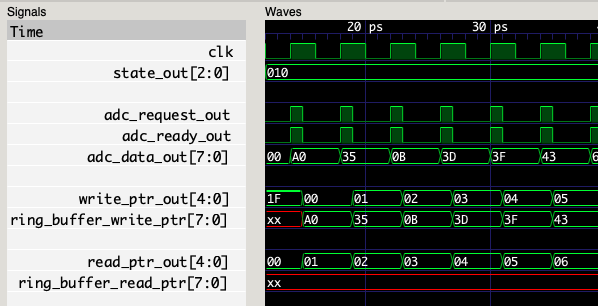
\includegraphics[width=\columnwidth]{Figures/Badc_ring_buffer_write}
    \caption{Ring Buffer Writing gktwave Output}
    \label{fig:testB}
\end{figure}

In RUNNING state, the adc value is written into the ring buffer.
As it is shown in \fref{fig:testB}, the first byte the ADC module is 0xA0 which is correctly written into address 0 of the ring buffer, and the second byte 0x35 is written into address 1 of the ring buffer, etc.
The byte at the read buffer pointer is unknown at it has not been written yet, and will only output a known value once a full loop of the ring buffer has been written.

\subsection{Ring Buffer Reading}
\begin{figure}[H]
    \centering
    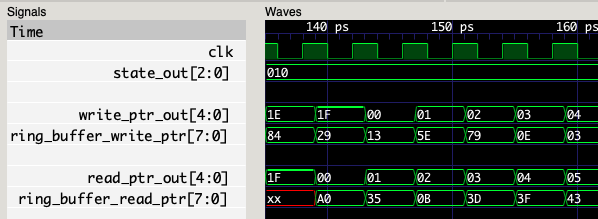
\includegraphics[width=\columnwidth]{Figures/Cadc_ring_buffer_read}
    \caption{Ring Buffer Reading gktwave Output}
    \label{fig:testC}
\end{figure}

As mentioned in \ssref{subsec:ring-buffer-writing}, a full loop has been written into the ring buffer and the read pointer is correctly return 0xA0 for address 0, and 0x35 for address 1, etc.

\subsection{Triggering}
\begin{figure}[H]
    \centering
    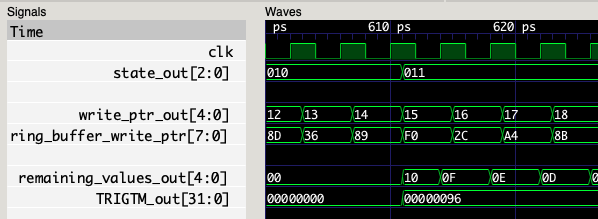
\includegraphics[width=\columnwidth]{Figures/Dtriggered}
    \caption{Triggering gktwave Output}
    \label{fig:testD}
\end{figure}
\begin{figure}[H]
    \centering
    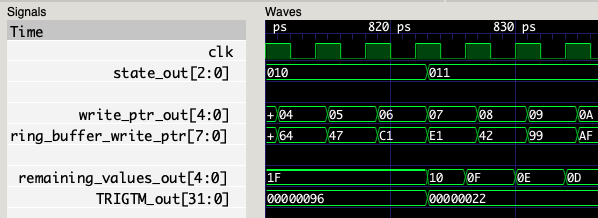
\includegraphics[width=\columnwidth]{Figures/Dtriggered2}
    \caption{Re-triggering gktwave Output}
    \label{fig:testD2}
\end{figure}

\fref{fig:testD} and \fref{fig:testD2} show an initial triggering and re-triggering of the TSC module respectively.
At the point of triggering, the state correctly changes to TRIGGERED (0b011) and the remaining ADC values is set to 16 to indicate that there are 16 more adc values to be written into the ring buffer.
The remaining values then starts counting down with every adc value saved to the ring buffer.
Additionally, the TRGRTM for the initial trigger is correctly updated to the current value of the timer which is:

$\frac{trigger\ time - start\ time}{clock\ period} = \frac{612ps - 12ps }{4ps} = 150 = \mathrm{0x96}$

\subsection{Raising TRD Line}
\begin{figure}[H]
    \centering
    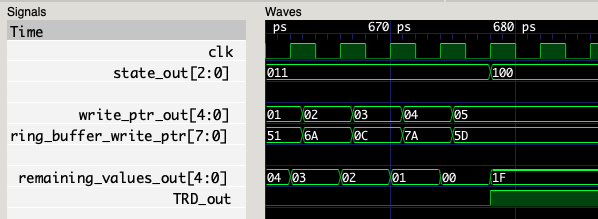
\includegraphics[width=\columnwidth]{Figures/E16captured}
    \caption{Raising TRD Line gktwave Output}
    \label{fig:testE}
\end{figure}

Once there are no remaining values (the remaining value register has reached 0), the TSC module correctly changes state to IDLE (0b100), stops recording adc values, and pulls the TRD line to the HUB module high.

\subsection{Starting or Transmitting From Idle}
\begin{figure}[H]
    \centering
    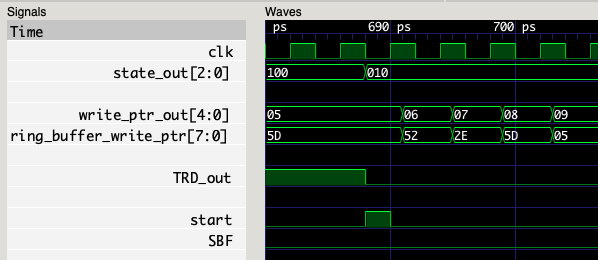
\includegraphics[width=\columnwidth]{Figures/Fidle_start}
    \caption{Starting From Idle gktwave Output}
    \label{fig:testF}
\end{figure}
\begin{figure}[H]
    \centering
    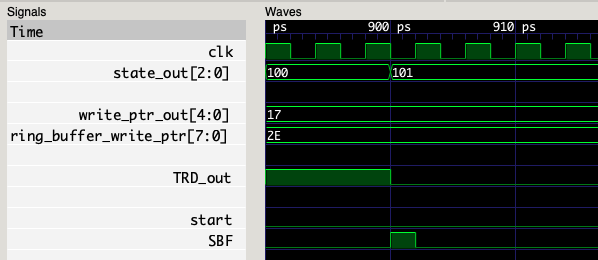
\includegraphics[width=\columnwidth]{Figures/Gidle_SBF}
    \caption{Transmitting Data From Idle gktwave Output}
    \label{fig:testG}
\end{figure}

From the IDLE state, the TSC module can either transition back to RUNNING or SENDING depending on the next command sent.
In \fref{fig:testF}, the TSC module receives a start pulse, correctly transitions back to RUNNING (0b010) state, and correctly continues writing the ADC values into the ring buffer.
In \fref{fig:testG}, the TSC module receives a SBF pulse, correctly transition into SENDING (0b101) state, and starts transmitting data with is shown in \ssref{subsec:starting-data-transmission}.

\subsection{Starting Data Transmission}\label{subsec:starting-data-transmission}
\begin{figure}[H]
    \centering
    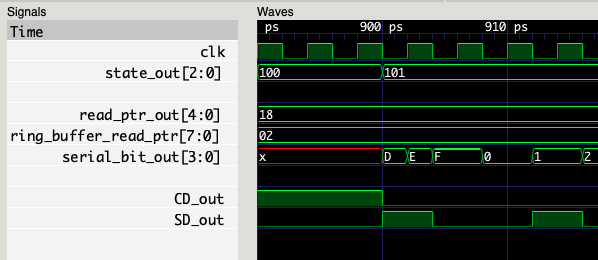
\includegraphics[width=\columnwidth]{Figures/Htransmit_start}
    \caption{Starting Data Transmission gktwave Output}
    \label{fig:testH}
\end{figure}

\subsection{Byte Transmitting}
\begin{figure}[H]
    \centering
    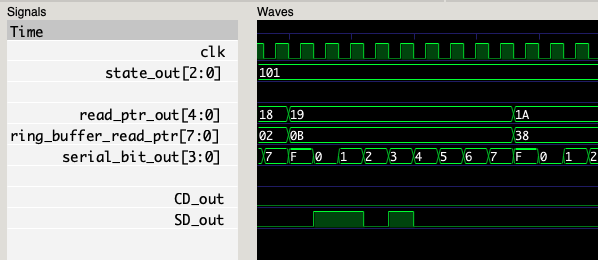
\includegraphics[width=\columnwidth]{Figures/Ibyte_transmit}
    \caption{Byte Transmitting gktwave Output}
    \label{fig:testI}
\end{figure}

\subsection{Ending Data Transmission}
\begin{figure}[H]
    \centering
    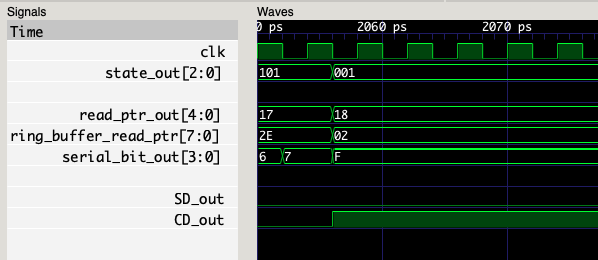
\includegraphics[width=\columnwidth]{Figures/Jtransmit_end}
    \caption{Ending Data Transmission gktwave Output}
    \label{fig:testJ}
\end{figure}

    \section{Conclusion}

The experiments show tha that small matrix sizes, single-threaded matrix multiplication is faster due to over heads.
As the matrix size increases, parallelized multiplication becomes quicker due to overhead becoming negligible relative to computation time.
The overhead includes OpenCL setup overheads and kernel startup overheads, with the former being constant and the latter increasing linearly with matrix count.
Due to the kernel startup overheads , parallelization efficiency improves slightly with larger matrix counts.
Overall, parallelized multiplication offers significant speedup for larger matrices compared to the single-threaded approach.

    %\bibliography{Bibliography/Bibliography}

\end{sloppypar}
\end{document}
